\clearpage
\bgroup
% Update the following macros to generate variants
% Also change the starting line number of the code

\newcommand{\elem}
{elem} % F18, Up to F18
%{char} % F18
%{string} % S19
\newcommand{\elemB}{\ifdefstring{\elem}{elem}{int}{\elem}}

\Question{Doubly-Linked Lists}

Consider the following interface for stacks that store
elements of the type \texttt{\elem}:

\begin{quote}
\begin{lstlisting}
// typedef ______* stack_t;

bool stack_empty(stack_t S)              /* O(1) */
/*@requires S != NULL; @*/ ;

stack_t stack_new()                      /* O(1) */
/*@ensures \result != NULL;      @*/
/*@ensures stack_empty(\result); @*/ ;

void push(stack_t S, [*\elem*] x)           /* O(1) */
/*@requires S != NULL; @*/ ;

[*\elem*] pop(stack_t S)                    /* O(1) */
/*@requires S != NULL;       @*/
/*@requires !stack_empty(S); @*/ ;
\end{lstlisting}
\end{quote}

Suppose we decide to implement the stack (of \texttt{\elemB}'s) using
a doubly-linked list so that each list node contains two pointers, one
to the next node in the list and one to the previous
(\lstinline'prev') node in the list:

\begin{center}
\ifdefstring{\elem}{char}{
  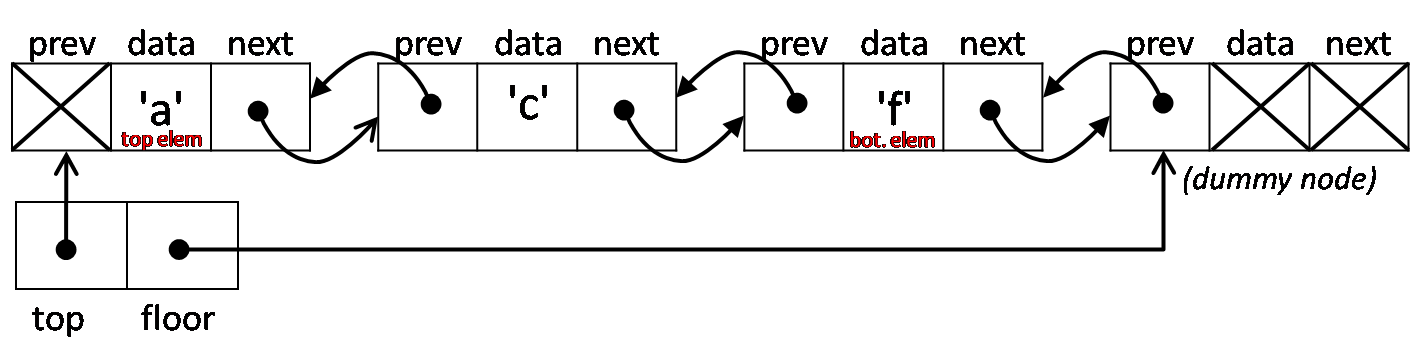
\includegraphics[width=0.9\linewidth]{\img/dll-char.png}
}{\ifdefstring{\elem}{string}{
  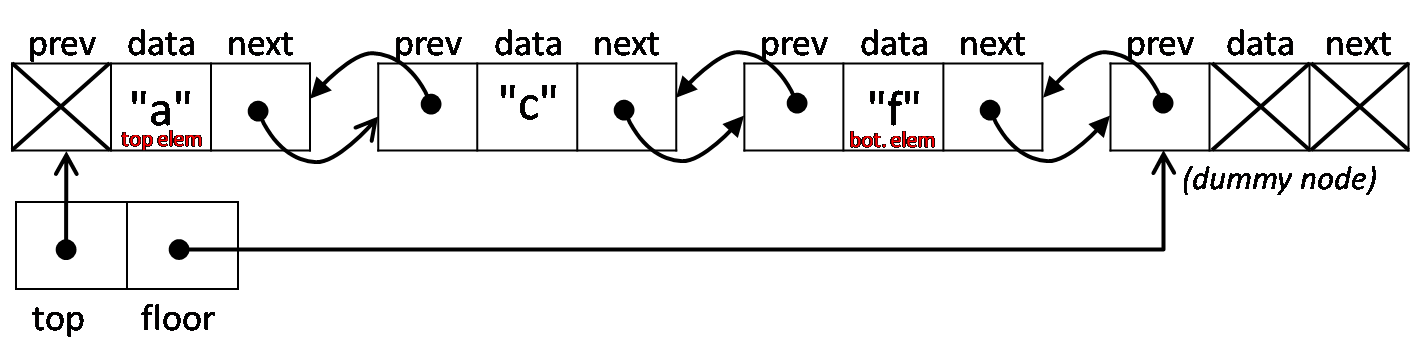
\includegraphics[width=0.9\linewidth]{\img/dll-string.png}
}{
  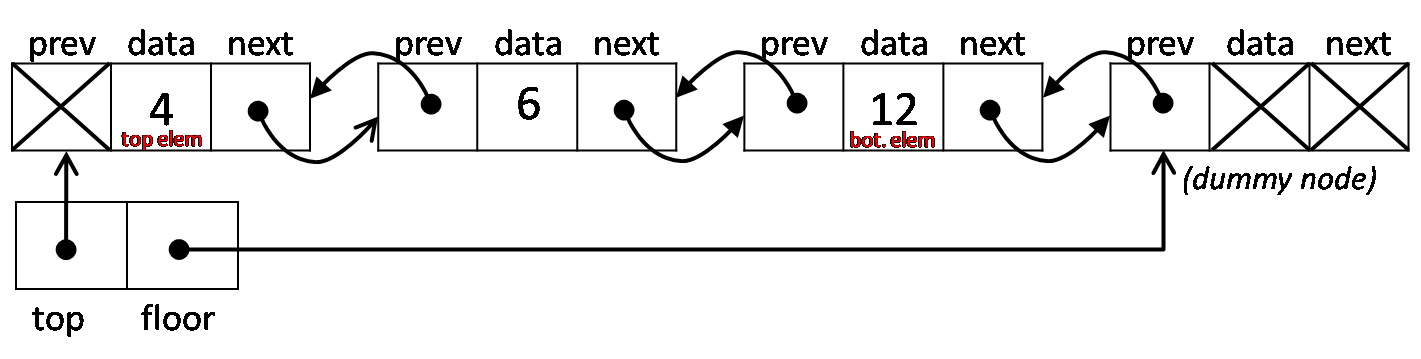
\includegraphics[width=0.9\linewidth]{\img/dll-int.png}
}}
\end{center}

\vspace{-1ex}
\begin{minipage}[t]{0.43\textwidth}
\begin{lstlisting}
typedef struct list_node list;
struct list_node {
  [*\elem*] data;
  list* prev;
  list* next;
};
\end{lstlisting}
\end{minipage}%
\rule[-17.5ex]{0.01em}{16ex}~
\begin{minipage}[t]{0.57\textwidth}
\begin{lstlisting}[showlines]
typedef struct stack_header stack;
struct stack_header {
  list* top;
  list* floor; // points to dummy node
};

\end{lstlisting}
\end{minipage}

%\enlargethispage{3ex}
The top element of the stack (if any) will be
stored in the first node of the list (pointed to by \lstinline'top'),
and the bottom element of the stack (if any) will be stored in the
second-to-last node in the list, with the last node being a ``dummy
node'' (pointed to by \lstinline'floor').  Intuitively, the bottom
element sits on the \lstinline'floor'.

An empty stack consists of a dummy node only: the \lstinline'prev',
\lstinline'data', and \lstinline'next' fields of that dummy are all
unspecified. A non-empty stack has an unspecified \lstinline'prev'
field for the top, and an unspecified \lstinline'data' and
\lstinline'next' field for the dummy node.

\begin{parts}

\part[2]\TAGS{linked-list, stack}
Modify the singly-linked list implementation of stacks given below to
work with the doubly-linked list representation given above. For each
function, either state the modification(s) that need to be made
(e.g. ``Insert the statement XXXX after line Y'', ``Remove line Z'',
``Change line Z to XXXX'', etc.) or state ``No change needs to be
made''. You may assume there is an appropriate \lstinline'is_stack'
specification function already defined. Be sure that your
modifications still maintain the O(1) requirement for the stack
operations.

\begin{lstlisting}[numbers=left, firstnumber=25, name=stack]
stack* stack_new()
//@ensures is_stack(\result);
//@ensures stack_empty(\result);
{
    stack* S = alloc(stack);
    list* L = alloc(list);
    S->top = L;
    S->floor = L;
    return S;
}

\end{lstlisting}
\begin{framed}
\ifprintanswers{\color{\answerColor}
  No changes need to be made.
}\else~\vspace{1.8in}\fi
\end{framed}

\RUBRIC
Part (a 1)
TAGS: linked-list, stack

Gradescope rubric:
+0.25pt No changes need to be made

Commentary:
- Line numbers change from semester to semester
- No change needs to be made: according to the description, the
  empty stack contains one dummy node with all fields unspecified.
ENDRUBRIC

\enlargethispage{5ex}
\begin{lstlisting}[numbers=left, name=stack]
bool stack_empty(stack* S)
//@requires is_stack(S);
{
    return S->top == S->floor;
}

\end{lstlisting}
\begin{framed}
\ifprintanswers{\color{\answerColor}
  No changes need to be made
}\else~\vspace{2.0in}\fi
\end{framed}

\RUBRIC
Part (a 2)

Gradescope rubric:
+0.25pt No changes need to be made

Commentary:
- Line numbers change from semester to semester
- No change needs to be made: according to the description, the
  empty stack contains one dummy node with all fields unspecified.
ENDRUBRIC

\newpage
\begin{lstlisting}[numbers=left, name=stack]
void push(stack* S, [*\elem*] x)
//@requires is_stack(S);
//@ensures is_stack(S);
{
    list* L = alloc(list);[*\label{l:dll-alloclist}*]
    L->data = x;
    L->next = S->top;
    S->top = L;[*\label{l:dll-Stop=L}*]
}

\end{lstlisting}
\begin{framed}
\ifprintanswers{\color{\answerColor}
  Insert \lstinline'S->top->prev = L' somewhere after
  line~\ref{l:dll-alloclist}.

  Or insert \lstinline'L->next->prev = L' after line~\ref{l:dll-Stop=L}.
}\else~\vspace{2.0in}\fi
\end{framed}

\RUBRIC
Part (a 3)

Gradescope rubric:
+0.5pt EITHER -- Insert S->top->prev = L somewhere after line [list* L = alloc(list)] and before [S->top = L]
+0.5pt OR -- Insert L->next->prev = L after [L->next = S->top]

Commentary:
- Line numbers change from semester to semester
ENDRUBRIC

\begin{lstlisting}[numbers=left, name=stack]
[*\elem*] pop(stack* S)
//@requires is_stack(S);
//@requires !stack_empty(S);
//@ensures is_stack(S);
{
    [*\elem*] e = S->top->data;
    S->top = S->top->next;
    return e;
}

\end{lstlisting}
\begin{framed}
\ifprintanswers{\color{\answerColor}
  No change is needed, though some reasonable modifications are possible.
}\else~\vspace{2.0in}\fi
\end{framed}

\RUBRIC
Part (a 4)

Gradescope rubric:
+0.5pt  No change is needed, though some reasonable modifications are possible.

Commentary:
- Line numbers change from semester to semester
- pop: No change is needed
OR pop: Insert line S->top->next->prev = NULL between [S->top = S->top->prev] and [return e]
ENDRUBRIC

\newpage
\part[1]\TAGS{complexity, linked-list, stack}
We wish to add a new operation \lstinline'stack_bottom' to our stack
\textbf{implementation} from the previous part.  Here's its interface
prototype:

\begin{quote}
\begin{lstlisting}
[*\elem*] stack_bottom(stack_t S)     /* O(1) */
/*@requires S != NULL && !stack_empty(S); @*/ ;
\end{lstlisting}
\end{quote}

This operation returns (but does not remove) the bottom element of the
stack.  Implement this function using the doubly-linked list
implementation of stacks from the previous part. Be sure that your
function runs in constant time. \emph{(Remember that the linked list
  that represents the stack has a dummy node.)}

\begin{framed}
\begin{lstlisting}[belowskip=0pt]
[*\elem*] stack_bottom(stack* S)
//@requires is_stack(S);
//@requires !stack_empty(S);
{
\end{lstlisting}
\ifprintanswers
\begin{lstlisting}[basicstyle=\basicstyle\color{\answerColor}]
  return S->floor->prev->data;
\end{lstlisting}
\else~\vspace{3.5in}\fi
\begin{lstlisting}[aboveskip=0pt]
}
\end{lstlisting}
\end{framed}

\RUBRIC
Part (b1)
TAGS: complexity, linked-list, stack

Gradescope rubric:
+0.5pt  EITHER -- return S->floor->prev->data
+0.25pt OR -- return S->floor->prev

Commentary:
  return S->floor->prev->data (1pt)
  return S->floor->prev (.5pt)
  return S->top... (or while loop) (0pt)
  return S->end->data (0pt)
ENDRUBRIC

%\part[1]\TAGS{complexity}
If we didn't add the \lstinline'prev' link to each node, how long
would it take to return the bottom element of the stack in big-O
notation for a list of $n$ elements? Why? \emph{(Note that there is
  still a dummy node at the end of the linked list.)}
\begin{framed}
\medskip
$O(\uanswer{12em}{$n$})$

\bigskip
Because \hfill\uanswer{30em}{we would need to traverse the whole list from
  the beginning.\hfill}

\bigskip
\uanswer{33.8em}{}
\end{framed}

\RUBRIC
Part (b2)
TAGS: complexity

Gradescope rubric:
+0.25pt  O(n)
+0.25pt  Justification

Commentary: O(n)
ENDRUBRIC

\newpage
\part[1\half]\TAGS{ds-invariant, linked-list, testing}
Now, consider the following broken implementation of
\lstinline'is_stack' for this stack implementation.

\begin{lstlisting}
bool is_segment(list* node1, list* node2) {
  if (node1 == NULL) return false;
  if (node1 == node2) return true;
  return is_segment(node1->next, node2);
}

bool is_stack(stack* S) {
  return S != NULL && is_segment(S->top, S->floor);
}
\end{lstlisting}

Draw a complete picture of a stack data structure (with
\texttt{\elemB} elements) that contains at least 4 allocated
\lstinline'list_node' structs and that returns \lstinline'true' from
\lstinline'is_stack' yet would not be well-formed.  \emph{Give
  specific values everywhere.  \textbf{Don't} use Xs anywhere; they
  are for unspecified values. So your diagram should depict pointers
  (possibly \lstinline'NULL') and values of type \texttt{\elem}.}  For full
credit your example struct must fail the unit test below with a
segfault or an assertion failure after passing the initial assertion.

\begin{framed}
\textbf{Stack picture:}
\ifprintanswers
\begin{lstlisting}[basicstyle=\basicstyle\color{\answerColor}, aboveskip=-0.7cm, belowskip=0pt]
                   .-----------------.@
              #    v     #           |
  +-----+    +|----+    +|-----+    +|----+
  |X|4|*|    |*|6|*|    |*|12|*|    |*|X|X|
  +----|+    +----|+    +-----|+    +-----+
   ^   |     ^    |     ^     |     ^^
   |   .-----.    .-----.     .-----.|
   |                                 |
   | .-------------------------------.
  +|-|+
  |*|*|                    #: anywhere
  +---+                    @: anywhere but a cell containing 12
\end{lstlisting}
\else~\vspace{2.1in}\fi
\end{framed}

\RUBRIC
Part (c)
TAGS: ds-invariant, linked-list, testing

Gradescope rubric:
+0.5pt At least 4 allocated list structs and clearly shows header node
+0.5pt Pass first assert
+0.5pt Fail unit test

Commentary:
Grade based on whether their example fails the unit test.
 - If they leave Xs anywhere, then make the xs concrete in the way
   that gives them the FEWEST points (this is called 'demonic
   non-determinism,' which I swear I didn't just make up -RJS)
 - Labels aren't critical as long as the structure is obvious
 - Grading
    * Half point for (at least) 4 allocated list structs
      and if they clearly draw the header node (they must label the
      top/bottom or start/end clearly, though, or they get no credit
      for the question)
    * Half a point for a correct counter example (if they draw a
    broken doubly-linked list that fails the unit test)

example answer:
                 .-----------------.@
            #    v     #           |
+-----+    +|----+    +|-----+    +|----+
|X|4|*|    |*|6|*|    |*|12|*|    |*|X|X|
+----|+    +----|+    +-----|+    +-----+
 ^   |     ^    |     ^     |     ^^
 |   .-----.    .-----.     .-----.|
 |                                 |
 | .-------------------------------.
+|-|+
|*|*|
+---+

#: anywhere
@: or anywhere but a cell containing 12

By the end of the loop:
x = 6
y = 12

ENDRUBRIC

\enlargethispage{5ex}
\begin{lstlisting}[belowskip=0pt]
// Unit test that your example above should fail
int main() {
    stack* S = // Code that constructs the example above.
               // By necessity, this won't respect the interface
    assert(is_stack(S) && !stack_empty(S)); // This must pass
    [*\elem*] x = stack_bottom(S);
    [*\elem*] y = pop(S);
    while (!stack_empty(S)) {
        y = pop(S);
        assert(is_stack(S));
    }
    assert(x == y);
    return 0;
}
\end{lstlisting}

\end{parts}

\egroup